\documentclass[11pt]{article}
\input{glyphtounicode}
\pdfgentounicode=1

\usepackage[utf8]{inputenc}
\usepackage[T1]{fontenc}
\usepackage{lmodern}
\usepackage{amsmath,amssymb}
\usepackage[margin=1in]{geometry}
\usepackage{booktabs}
\usepackage{multirow}
\usepackage{array}
\newcolumntype{L}[1]{>{\raggedright\arraybackslash}p{#1}}
\usepackage{graphicx}
\usepackage[section]{placeins}
\usepackage[sort]{natbib}
\setlength{\bibsep}{4pt}
\bibliographystyle{apalike}
\usepackage{caption}
\captionsetup{font=small}
\usepackage[hidelinks]{hyperref}
\usepackage{setspace}
\setstretch{1.13}
\widowpenalty=10000
\clubpenalty=10000
\renewcommand{\topfraction}{0.9}
\renewcommand{\bottomfraction}{0.6}
\renewcommand{\textfraction}{0.07}
\renewcommand{\floatpagefraction}{0.8}
\newcommand{\pinc}{\overline{\mathrm{ParentInc}}}

\title{Before the Labor Market or Inside It?\\
Family Background, Earnings Dynamics, and the Return to College}
% The one place to set the address of the public repository (online appendix and replication files).
\newcommand{\repourl}{https://github.com/JiachenJin1001/family-background-earnings-china}
\author{Jiachen Jin\thanks{New York University, \texttt{jj4608@stern.nyu.edu}.
The Online Appendix (supplementary results, proofs of the formal results, and a replication guide) and the replication files are available at \href{\repourl}{\nolinkurl{github.com/JiachenJin1001/family-background-earnings-china}}.
All errors are mine.}}
\date{November 2026}

\hypersetup{pdftitle={Before the Labor Market or Inside It? Family Background, Earnings Dynamics, and the Return to College}, pdfauthor={Jiachen Jin}}
\begin{document}
\maketitle

\begin{abstract}
\noindent In the China Family Panel Studies, the children of officials, managers, and
professionals (advantaged children) earn 22 percent more than other
children (less advantaged children). I ask whether this advantage is
built inside the labor market, through smaller earnings shocks or
faster earnings growth, or is already in place before work begins, through access to college, and I find the latter.
Covariance-structure and panel estimates show no difference between the two groups' earnings processes: lasting differences and transitory shocks are the same size, shocks fade at the same rate, and earnings grow at the same rate. Parental income, held fixed by correlated random-effects regressions and by entropy balancing, accounts for one fifth to three fifths of the gap; the remaining premium of 7 to 17 percent is what parental occupation carries beyond income. To learn whether the premium runs through college, I estimate the return to college from the 1999 expansion of university admissions, using an instrument that interacts provincial growth in university seats with birth-cohort exposure. The added seats gave children in both groups a similar chance of entering college, and for children who entered because of them, college raised earnings by 0.68 log points, or 19 percent per year of college. A degree also closes the occupational gap between the groups. The point estimates suggest a higher earnings return to college for advantaged children, while for less advantaged children college brings a larger rise in the chance of holding an advantaged occupation. What parental occupation passes on beyond income is thus mostly a four-year degree: valued at the return to college, the gap in college completion accounts for three quarters to all of the premium.\\[4pt]
\textbf{JEL:} J62, J31, I23, I24, C23. \quad \textbf{Keywords:}
intergenerational mobility; earnings dynamics;
attenuation bias; higher
education expansion; shift-share instrument; China.
\end{abstract}

\newpage

\section{Introduction}
\label{sec:intro}

In the China Family Panel Studies (CFPS), children with a parent in an official, managerial, or professional occupation (advantaged children) earn 22 percent more than other children (less advantaged children). Part of that gap reflects parental income: holding parental income and demographics fixed removes one fifth to three fifths of it. What remains, a premium of 7 to 17 percent (0.07 to 0.15 log points), is not accounted for by the family's measured income. What do these parents pass on beyond income? It could be an advantage that accumulates over a career: their children might face smaller earnings shocks, recover from bad years faster, or climb steeper career paths. Or it could be in place before work begins, if what these families secure is schooling, above all a place at university. The data support the second. Once at work, the two groups' earnings behave alike: shocks are the same size and fade at the same rate, and earnings grow at the same rate. Most of the premium runs through college, which is completed before work begins.

Behind this premium lies the question of social mobility: whether the chance to move up, in earnings and in occupation, is open to less advantaged children. The answer bears on how a society uses its talent and on how its members view redistribution \citep{AlesinaStantchevaTeso2018, BellEtAl2019, HsiehHurstJonesKlenow2019}. Where the advantage arises also determines what can change it: protection inside the labor market would operate throughout a career, and no single reform at the start of adult life could undo it, whereas an advantage settled at the university gate depends on the rules that allocate seats.

I measure the premium beyond parental income (Section~\ref{sec:premium}) on the level of earnings at ages 30 and over, by correlated random-effects regressions and by entropy balancing, which reweights less advantaged children to match the parental income and demographics of advantaged children. The two ends of its range come from two measures of parental income, one that over-controls and one that under-controls. Party membership and state-sector employment, two other markers of position, add little once parental occupation is included.

The first place to look for the source of the premium is the labor market, and the test is the earnings process (Section~\ref{sec:process}). If these parents protect their children's earnings, the protection should appear in the variance of earnings or in earnings growth: smaller shocks, shocks that fade faster, or steeper earnings paths. For the 2,523 children observed in at least three waves I estimate the process of residual earnings for each group and for both together: a permanent--transitory model fitted by minimum distance to the autocovariances, an Arellano--Bond dynamic panel regression for the persistence of shocks, and a fixed-effects regression for growth. The two groups share one process. When I impose the same permanent variance, shock variance, and persistence on both groups and then free them, each parameter freed on its own differs by less than one standard error, and freeing all three improves the fit by no more than sampling variation would; nor does the earnings gap between the groups grow over the panel. The process resembles the one found in U.S. panels: the permanent component is about a quarter of the variance of residual earnings, so a regression on a single wave of income recovers only about a quarter of the coefficient on permanent income (Section~\ref{sec:measurement}), the errors-in-variables problem of \citet{Solon1992}. The estimated process is used twice more: it supplies the attenuation factor for every comparison that holds parental income fixed and the precision weights for the return to college, so the measurement result and the causal estimate rest on the same parameters.

Since the earnings process offers no source for the premium, the second place to look is college (Sections~\ref{sec:expansion} and \ref{sec:mediation}). Whether the premium runs through college depends on the return to college, which least squares does not identify, because college completion is endogenous: children who complete college differ from those who do not in ability, preparation, and family resources that raise earnings on their own. Identifying the return takes a change in access to college that no family chose, and the 1999 expansion is one: university admissions rose by more than 40 percent in a single year and kept growing for a decade, at rates that differed across provinces. To separate the reform from the national trend in admissions I use a shift-share instrument for college completion: a provincial measure of how much university seats grew (provincial intensity), multiplied by the exposure of each birth cohort, the ratio of national admissions in the year the cohort reached college age to the pre-reform trend. With province and birth-year fixed effects, the comparison is a difference-in-differences between provinces that added more and fewer seats and between cohorts that were more and less exposed.

Two-stage least squares on this comparison identifies the return to college for children who entered college because of the added seats. For these children the instrumented return is 0.68 log points, or 19 percent per year of college, and it is about the same when each child's average earnings are weighted by the precision that the earnings process of Section~\ref{sec:process} implies. College also opens official, managerial, or professional occupations (advantaged occupations): the instrumented estimate is that it raises the chance of holding one by 0.50. Advantaged children are twice as likely as less advantaged children to hold one (0.33 against 0.17), and the same is true among children without a degree (0.19 against 0.10); with a degree, both groups reach 0.60. Among children who entered college because of the reform, the point estimates suggest a higher earnings return to college for advantaged children (1.14 against 0.62 log points) and a larger rise in the chance of holding an advantaged occupation for less advantaged children (0.55 against 0.13).

The design rests on two assumptions: parallel trends (provinces that added more seats were not already on different trends) and exclusion (the instrument affects the outcomes only through college). Four of the checks in Section~\ref{sec:expansion} bear them out. A predetermined provincial measure, the census share of adults who had completed senior secondary school before the reform, reproduces the earnings results. A placebo built from pre-reform growth in examination registrations, which I assemble from statistical yearbooks, has no first stage. Children with nine or fewer years of schooling, who were never candidates for college, did not move into official, managerial, or professional occupations where seats grew faster. Controls for the export boom that followed WTO accession leave the results unchanged.

The other half of the college channel is the gap in college completion. Between the cohorts born in 1980 or earlier and those born later, completion rose from 17.3 to 50.5 percent among advantaged children and from 4.6 to 24.2 percent among less advantaged children. The first stage shows that the added seats gave children in both groups a similar chance of entering college (18 percentage points for less advantaged children and 15 for advantaged children, between the 10th and 90th percentiles of intensity in the most exposed cohorts).

The return and the gap together account for the premium (Section~\ref{sec:mediation}). The premium $\tau$ equals the completion gap between children of the two groups with the same parental income, $\Delta M$, valued at the return to college for advantaged children, $\beta^{H}$, plus a direct effect:
\begin{equation}
\tau \;=\; \beta^{H} \cdot \Delta M \;+\; \mathrm{Direct}.
\label{eq:hp-intro}
\end{equation}
The direct effect is what reaches earnings without passing through college completion: information, connections, and any higher value that the same degree carries for an advantaged child. In the entropy-balanced comparison the premium is 0.072 log points (7 percent) and the completion gap is 12.2 percentage points. Valued at the estimated returns to college, the gap accounts for between three quarters and all of the premium. What parental occupation passes on beyond income is, for the most part, a four-year degree.

The gap in college completion can be read in two ways. Admission was by examination score alone, and the score may have ranked ability alone or preparation under unequal conditions: city schools, key-point high schools, and the material security to devote oneself to the examination. If it ranked only ability, children admitted from below the old cutoff would earn less from a degree than earlier graduates did, least squares would overstate the return, and removing that selection should lower the estimate. If it ranked preparation, they would earn as much from a degree or more. The instrumented return of 0.68 is above the least squares return of 0.45, which is consistent with the preparation hypothesis.

A natural reading of the premium is that advantaged parents pass on their ability. If so, advantaged children should out-earn less advantaged children with the same schooling, and advantaged graduates should reach advantaged occupations more often. Yet with parental income held fixed, children without a degree earn the same in the two groups, the earnings gap among graduates is small (Section~\ref{sec:mediation}), and graduates of the two groups are equally likely to hold advantaged occupations (Section~\ref{sec:earnings}). Most of the premium therefore comes through access to college, not through ability rewarded outside it.

The estimates of the residual earnings process apply covariance-structure methods \citep{LillardWillis1978, MaCurdy1982, HallMishkin1982, AbowdCard1989, MeghirPistaferri2004, ArellanoBlundellBonhomme2017} to the CFPS panel. The process looks the same in the two groups, which leaves earnings risk without a measurable role as a channel of transmission. To the measurement literature that began with \citet{Solon1992} and \citet{Zimmerman1992} and was extended by \citet{Mazumder2005} and \citet{HaiderSolon2006}, I add attenuation factors estimated on Chinese earnings, which the debate over persistence in China \citep{GongLeighMeng2012, DengGustafssonLi2013, FanYiZhang2021, YuanLin2013} has lacked. The work on China's college expansion has concentrated on the labor market for graduates, firms, and general-equilibrium effects \citep{CheZhang2018, KnightDengLi2017, Ma2024IER}, and on college entry, where family background kept its hold \citep{Yeung2013}, as the maximally maintained inequality hypothesis of \citet{RafteryHout1993} predicts. I ask which children the reform brought into college and what college returned to each group. 

\section{Data}
\label{sec:data}

\subsection{Panel and income concept}
\label{sec:income}

The China Family Panel Studies (CFPS) is a biennial household panel run by the Institute of Social Science Survey at Peking University since 2010 \citep{XieHu2014}. With its sampling weights, the baseline sample of 25 provinces represents about 95 percent of the national population; respondents who move are followed, and the sample of Section~\ref{sec:sample} spans 29 provinces. Because the sample conditions on panel participation, the sampling weights no longer reproduce the population; I do not use them, and the estimates describe the sample.

Before 2014 the survey's headline income variable bundles labor earnings with transfers and asset income; from 2014 onward it covers labor income only. An estimator that pooled waves across the change would attribute it to earnings shocks, so the main analysis uses the five waves from 2014 to 2022. For the growth-rate tests I reconstruct a labor-income measure for 2010 and 2012 from its components (the reconstructed panel); no main estimate rests on it.

\subsection{Sample and family background}
\label{sec:sample}

A child is a CFPS respondent linked to a father or mother through the family-relationship roster. The grouping variable, denoted $H_i$, equals one if either parent held an occupation in the top two major groups of China's Standard Classification of Occupations (CSCO): heads of state organs, party organizations, enterprises, and public institutions, or professionals and technical personnel, the counterparts of major groups 1 and 2 of the international classification, ISCO. Parental occupation is measured when the child was fourteen, from retrospective questions asked in the 2012, 2020, and 2022 waves, under the either-parent dominance convention of \citet{EriksonGoldthorpe1992}. Children with $H_i = 1$ are the advantaged children, and all others the less advantaged children. Occupation marks family position in these cohorts because the parents built their careers in the 1980s and 1990s, when state pay scales compressed wages and a parent's occupation determined the work unit, and with it housing, urban registration, and the connections that a post in government, management, or the professions carried \citep{BianLogan1996, WuTreiman2007}.

The paper uses a single sample. A child belongs to it if the data contain a retrospective report, the family income of the parental household, a province for which Section~\ref{sec:expansion} has a measure of the expansion, and positive labor income in at least two waves between 2014 and 2022 at ages 22 to 55 (22 is the age at which a four-year graduate enters the labor market, 55 the middle of the three statutory retirement ages). Wave by wave I drop log incomes below $\log 1000$ yuan and the top 1 percent of log income. The sample has 4,536 children (755 advantaged, 16.6 percent) and 12,675 child-waves, born 1961 to 1997.

Section~\ref{sec:process} studies earnings dynamics, and dynamic panel estimation requires at least three waves; 2,523 children (420 advantaged) have them. Sections~\ref{sec:premium}, \ref{sec:expansion}, and \ref{sec:mediation} study the level of earnings. A child's \emph{level of earnings} is the mean, over at least two waves at ages 30 and over, of log labor income net of survey-year effects; 2,774 children (453 advantaged) have one. Section~\ref{sec:expansion} keeps all 4,536 children; the 1,762 without a level of earnings enter the expansion regression in a second row built from their earnings before age 30, which helps estimate its province and birth-year effects and the coefficients on its controls (Section~\ref{sec:design}).

The definition involves two choices. The first is the threshold at age 30. Earnings in the twenties are a poor measure of where a career settles \citep{HaiderSolon2006}, and especially so here, because graduates enter the labor market later than other children: at ages 26 to 29 they are in their first years of work, while children of the same age without a degree have worked for about a decade. Controlling for survey-year and age effects, the least squares return to college is 0.37 log points at ages 26 to 29 and 0.46 at 30 to 34. The second is the removal of survey-year effects before averaging, because nominal incomes rose steeply over the panel and an average of raw log income would depend on the years in which a child happens to be observed; the effects are estimated on all child-waves and centered on the overall mean, so the result stays in log yuan.

Selection into the sample is nearly the same in the two groups: of the children with a retrospective report and parental family income who are observed at least once at ages 22 to 55 in a 2014--2022 wave, 45 percent of advantaged children satisfy every screen and enter the sample, against 42 percent of less advantaged children. Employment does differ: before any earnings screen is applied, earnings are positive in 56 percent of the person-waves of advantaged children and in 50 percent of those of less advantaged children, so the comparison of earnings risk is conditional on having earnings.

CFPS also records the occupations that parents hold from 2010 to 2022, which yields an indicator based on current occupations. The two measures agree for 86 percent of the children for whom both exist, and the disagreement runs in the direction retirement predicts, with more parents moving down by the observation window than up (10.2 against 4.0 percent of children). A measure taken after parents have retired or moved down misclassifies some advantaged families, so the retrospective indicator is the baseline; the other enters the robustness checks of Section~\ref{sec:premrobust}.

Table~\ref{tab:desc} compares the two groups, among all children in the sample and among the children with a level of earnings. In both, advantaged children earn about 0.2 log points more on average; they have parents with more family income (by more than 0.4 log points), acquire more than two additional years of schooling, and complete college at more than twice the rate of less advantaged children. They are more urban and more often female; birth years and the number of waves are balanced across the groups.


\begin{table}[t]
\centering
\small
\caption{Sample means by family background.}
\label{tab:desc}
\setlength{\tabcolsep}{5pt}
\begin{tabular}{@{}lcccc@{}}
\toprule
& \multicolumn{2}{c}{All children, ages 22 to 55} & \multicolumn{2}{c}{With earnings at ages 30 and over} \\
\cmidrule(lr){2-3}\cmidrule(lr){4-5}
& Advantaged & Less advantaged & Advantaged & Less advantaged \\
\midrule
Mean log labor income & 10.66 (0.65) & 10.45 (0.65) & 10.67 (0.64) & 10.48 (0.64) \\
$\pinc$ (log family income) & 10.99 (0.77) & 10.56 (0.74) & 11.06 (0.75) & 10.58 (0.79) \\
Years of schooling & 13.77 (3.08) & 11.56 (3.64) & 13.20 (3.32) & 10.74 (3.70) \\
College (16$+$ years) & 0.41 (0.49) & 0.18 (0.39) & 0.34 (0.47) & 0.14 (0.35) \\
Female & 0.36 (0.48) & 0.27 (0.45) & 0.30 (0.46) & 0.20 (0.40) \\
Urban (first wave) & 0.76 (0.43) & 0.55 (0.50) & 0.77 (0.42) & 0.56 (0.50) \\
Age (mean over waves) & 34.2 (8.6) & 34.1 (8.2) & 39.7 (7.0) & 39.2 (6.6) \\
Birth year & 1984.4 (9.0) & 1984.4 (8.5) & 1979.1 (7.7) & 1979.6 (7.2) \\
Waves with labor income & 2.81 (0.84) & 2.79 (0.83) & 2.75 (0.82) & 2.70 (0.80) \\
\addlinespace
Children & 755 & 3,781 & 453 & 2,321 \\
\bottomrule
\end{tabular}

\par\smallskip
\begin{minipage}{0.92\textwidth}
\footnotesize\emph{Notes:} Standard deviations in parentheses. CFPS
2014--2022. All children: the 4,536 children with at least two waves of
positive labor income at ages 22 to 55; their labor income is the mean
of log nominal annual income in yuan over all their waves. Children
with earnings at 30 and over: the 2,774 with at least two
waves at those ages; their labor income is the level of earnings
defined in the text (net of survey-year effects, centered on the overall mean), and age and the number of waves refer to the waves
at 30 and over. Advantaged: either parent held a CSCO major group 1 or
2 occupation when the child was fourteen.
\end{minipage}
\end{table}

\subsection{Parental income and co-residence}
\label{sec:parentinc}

Parental economic resources are measured as $\pinc_i$, the mean of log family income across all waves in which the parental household appears in the family-economy module. Family income covers more parents and more waves than the parents' labor income, since many parents are past working age, and it includes asset and business income. It has one known defect: when an adult child appears on the same household roster as a linked parent (nearly two thirds of the child-waves in the sample), it mechanically includes the child's own earnings, so a regression of child earnings on $\pinc_i$ partly regresses the child on herself. I therefore report a second measure built from the linked parents' own labor-income records. If co-residence contaminates the family measure, replacing it should lower the income coefficient and raise the occupation coefficient, and it does both (Section~\ref{sec:cre}).

\subsection{The 1999 expansion and provincial intensity}
\label{sec:background}

Through the 1990s, admission to Chinese universities was rationed by score on the national college entrance examination under a centrally planned enrollment quota that grew slowly, from roughly 0.7 million admissions in 1988 to one million in 1997, while candidates far outnumbered seats. For most students the binding constraint was the number of seats rather than the willingness to take the examination. The cost of competing for a seat also varied with family circumstance: opportunity costs
were high even where tuition was low, provincial admission cutoffs
differed, and urban schools prepared students better for the
examination.

In June 1999, after registration for that year's entrance examination
had closed, the central government announced a second and larger increase in that year's admissions \citep{LiWhalleyXing2014}; admissions grew by more than 40 percent in 1999 and passed five million by 2005. The trigger was
macroeconomic as much as educational, and the proposal moved from
memorandum to decision within months. Provinces had little time to fit seats to local demand for skill, and seats grew where existing institutions could add
them, on a timetable set in Beijing. 

By 1997 every institution charged tuition \citep{DongWan2012}, so the reform relaxed the seat
constraint while prices stayed positive, and the marginal student it
admitted had to clear a resource bar as well as the examination bar.
Admission operated through provincial quotas set institution by
institution, and a national percentage increase translated into different
seat growth across provinces depending on where seats could
be added; that administrative fact is the source of the cross-province
variation the design uses. The intensity measure defined below accordingly counts the
seats that institutions located in a province added, not the seats
allotted to the province's own candidates. The two nearly coincide:
institutions set their admission plans province by province and
reserve the largest share for the province in which they are located,
so a child, who takes the examination in the home province, competes
mainly for the seats of that province's institutions. The expansion grew the four-year (\emph{benke}) and three-year (\emph{dazhuan}) tiers of higher education at different provincial rates; college completion throughout means sixteen or more
years of schooling, the four-year degree.

Children born in 1981 or later reached age eighteen in the expansion
era. The 1981 cohort was admitted under the enlarged quota without
having planned for it, because registration for 1999 had closed before
the announcement; the first cohort able to plan around the policy took
the examination in 2000. The cohort dimension of the instrument is the
ratio of actual national admissions in the year a cohort turned
eighteen to a linear projection of the pre-reform trend, both computed from the national admissions series in \citet{Ma2024IER}. The ratio lies between 0.9 and 1.6 for the cohorts born 1964 to 1976, because admissions rose above the linear trend in the mid-1980s and fell back below it around 1990, and between 1.02 and 1.05 for those born 1977 to 1980; it rises to 1.44 for the 1981 cohort and reaches 4 for the cohorts born around 1990. Exposure enters
continuously, and the birth-year effects of the specification absorb
the level break together with every other common cohort movement.

Provincial intensity follows \citet{Ma2024IER}. The main measure is the
number of college graduates of 2006 to 2010 that the province's institutions are predicted to produce, divided by the province's
stock of college-educated workers in 2005. The prediction allots the national number of graduates to cities by their shares of national college enrollment in the 1982 census, because the expansion scaled up the institutions that already existed, and counts graduates where they studied. Two other normalizations of the same predicted inflow, by total employment in 2005 and as the log of the implied growth of the college-educated stock, serve as checks.
The enrollment shares were fixed long before the reform, but the denominators are measured in 2005, after it had begun. The analysis therefore also uses a
measure that is predetermined in every component, the census share of each province's
adults born 1956 to 1976 who had completed senior secondary school. The
share describes the size of the province's education system before the
reform, was fixed at least five years before it, is stable
across censuses (correlation 0.97 between the 1990 and 2000
measurements), and correlates 0.44 with the main measure across provinces. Statistical yearbooks supply a placebo: the growth of college entrance examination (CEE) registrations before the reform,
$\log(\mathrm{CEE}_{1998,p} / \mathrm{CEE}_{1997,p})$, which is upstream of admissions and predetermined. Interacted with cohort exposure, it should not predict college completion if the design isolates the reform rather than generic provincial trends.

\section{The premium}
\label{sec:premium}

I measure the premium on the level of earnings defined in Section~\ref{sec:sample}, for the 2,774 children who have one. Before any controls, advantaged children earn 0.195 log points (22 percent) more than less advantaged children, and 34 percent of them completed college, compared with 14 percent. Parental income and the demographic controls, held fixed by regression (Section~\ref{sec:cre}) and by reweighting (Section~\ref{sec:ebal}), remove a fifth to three fifths of the raw gap of 0.195. The rest, 0.07 to 0.15 log points or 7 to 17 percent, is the premium: an association, net of current family resources, rather than a causal effect.

I leave two variables out of the regressions because they would be bad controls \citep{AngristPischke2009, AcharyaBlackwellSen2016}. One is parental education: in these parental cohorts, born mostly between the late 1930s and the early 1970s, schooling was interrupted and reallocated on political criteria, so credentials were in large part consequences of political and occupational position. The other is the child's own education, the channel that Sections~\ref{sec:expansion} and \ref{sec:mediation} study.

\subsection{Correlated random-effects estimates}
\label{sec:cre}

The main specification is a correlated random-effects (Mundlak)
regression \citep{Mundlak1978},
\begin{equation}
\log y_{it} \;=\; \delta_1 H_i \;+\; \delta_2\, \pinc_i \;+\; x_{it}'\gamma \;+\; \bar x_i'\xi \;+\; z_i'\kappa \;+\; \phi_t \;+\; \mu_p \;+\; u_{it},
\label{eq:cre}
\end{equation}
with $x_{it}$ the time-varying controls (age, urban status), $\bar x_i$
their within-child means, $z_i$ the time-invariant controls (gender), $\phi_t$ and $\mu_p$ year and province effects, and standard errors clustered on person; $\delta_1$ estimates the premium
$\tau$. Table~\ref{tab:cre} shows what conditioning on parental resources does to the occupation coefficient. Adding family income lowers the coefficient from 0.163 to 0.088, by nearly half ($p = 0.002$). Replacing the family measure with the parents' own labor income, on the 2,185 children whose parents report it, moves
both coefficients in the direction that co-residence contamination
predicts: the income coefficient falls from 0.222 to 0.031 and the occupation coefficient rises to 0.153 ($p < 0.001$). The two columns err in opposite directions, so they bracket the premium. Column 1 over-controls, because family income contains the child's own earnings when the child lives with the parents. Column 2 under-controls: the parents' labor income leaves out asset and business income and is observed only in waves in which a parent works, so by the schedule of Section~\ref{sec:measurement} its coefficient is attenuated and it holds less of the family's resources fixed. The regression-based premium therefore lies between 0.088 and 0.153 log points (9 and 17 percent).

\begin{table}[t]
\centering
\small
\caption{The premium net of parental income: three estimates.}
\label{tab:cre}
\begin{tabular}{@{}>{\raggedright\arraybackslash}p{5.6cm}ccc@{}}
\toprule
& (1) & (2) & (3) \\
Estimator & Correlated & Correlated & Entropy \\
& random effects & random effects & balancing \\
Parental income measure & Family income & Parental labor income & Family income \\
\midrule
\multirow[t]{2}{=}{Advantaged, $H$ (parent in CSCO major groups 1 or 2 at child age 14)} & 0.088\rlap{***} & 0.153\rlap{***} & 0.072\rlap{**} \\
 & (0.029) & (0.034) & [0.01, 0.13] \\
\multirow[t]{2}{=}{Coefficient on parental income} & 0.222\rlap{***} & 0.031\rlap{***} & --- \\
 & (0.016) & (0.011) &  \\
Children & 2,774 & 2,185 & 2,774 \\
\bottomrule
\end{tabular}

\par\smallskip
\begin{minipage}{0.92\textwidth}
\footnotesize\emph{Notes:} Dependent variable: log annual labor income
by child and wave (columns 1 and 2) and the level of earnings (column
3). Columns 1 and 2: correlated random-effects regressions on the child-waves at ages 30 and over of the 2,774 children with a level of earnings (column 2: the 2,185 of them whose parents report labor income), standard errors clustered on person, controls for
age, year and province fixed effects, gender, urban status, and
within-child means of the time-varying covariates. Clustering at the family level instead changes the column 1 standard error by 0.0002 (159 of the 2,606 families have two or more of these children). Column 3: less advantaged children reweighted to match the first two
moments of parental income, gender, age, urban status, five-year birth cohort, and province (the fifteen largest separately) among advantaged children (equation~\eqref{eq:ebal}); the
bracket is a 200-replication bootstrap percentile interval.
*, **, and *** denote significance at the 10, 5, and 1 percent levels; the balancing estimate carries ** when its 95 percent bootstrap interval excludes zero.
\end{minipage}
\end{table}

\subsection{Entropy balancing}
\label{sec:ebal}

Entropy balancing \citep{Hainmueller2012} estimates the same premium by a different route and fits no earnings equation. It reweights the whole
group of less advantaged children so that their weighted means and variances
of parental income, gender, age, urban status, five-year birth cohort, and province (the fifteen largest separately)
equal those of advantaged children exactly. The weights $w_i$ solve
\begin{equation}
\min_{w} \sum_{i:\, H_i = 0} w_i \log w_i
\quad\text{subject to}\quad
\sum_{i:\, H_i = 0} w_i\, g(x_i) = \frac{1}{N_1}\sum_{j:\, H_j = 1} g(x_j),
\quad \sum_{i:\, H_i = 0} w_i = 1,
\label{eq:ebal}
\end{equation}
where $g(x)$ collects the covariates and their squares and $N_1$ is the number of advantaged children; the weights stay as
close as possible to uniform weights while balancing the moments, and
the premium is the difference between the advantaged mean of log
earnings and the weighted mean of less advantaged children. The balanced difference in mean log
earnings is 0.072, or 7 percent, with a 200-replication bootstrap percentile interval of $[0.01, 0.13]$. Under the same weights the
gap in college completion between the groups is 0.122, or 12.2 percentage points (interval $[0.08, 0.17]$). Both figures are for all 2,774 children, the cohorts before and after the reform together. Regression and balancing condition on the same observables and neither addresses unobserved confounding, but with the same income measure they give nearly the same premium, 0.088 and 0.072.

\subsection{Competing markers and robustness}
\label{sec:class}
\label{sec:premrobust}

If parental occupation proxies for social position broadly, other markers of position should add little once it is included. Two natural competitors are parental party membership \citep{LiEtAl2007} and employment inside the state system, both between two and three times as common among the parents of advantaged children. In regressions of the level of earnings with parental income and the demographic controls (Online Appendix), each marker alone carries a coefficient a little over half that of parental occupation and is not distinguishable from zero. Once parental occupation is added, the marker coefficients fall by roughly a third while the occupation coefficient barely moves. A post in government, enterprise management, or the professions was usually a post inside the state system, and party membership was a common step in the career that led to one, so parental occupation already records what the two other markers measure.

Figure~\ref{fig:spec} reports thirteen specifications, which vary the income control, the definition of the indicator, the estimator, the province effects, and the deflator. Ten of the thirteen estimates lie between 0.06 and 0.09, and ten intervals exclude zero; the range runs from 0.057, with CSCO major group 1 alone as the indicator, to 0.153, with the parents' own labor income as the income control. The Online Appendix adds the urban and rural subsamples.

\begin{figure}[t]
\centering
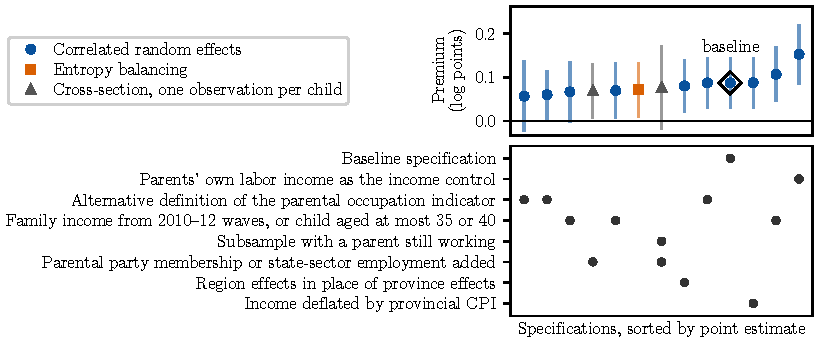
\includegraphics[width=0.84\textwidth]{figures/fig_spec_curve_paper}
\caption{The premium in thirteen specifications, sorted by point estimate. Vertical bars are 95 percent confidence intervals; the diamond marks the baseline; the lower panel marks the analytic choices in each specification.}
\label{fig:spec}
\end{figure}

The indicator based on current occupations, measured after the formative years, gives a smaller estimate, 0.049 ($p = 0.27$), which is what misclassification predicts. A misclassified binary regressor cannot carry classical measurement error, because the error is necessarily negatively correlated with the true value. If misclassification is nonetheless unrelated to the child's outcome and to the controls, it can only shrink the coefficient, in the simplest case by one minus the sum of the two misclassification rates \citep{Bollinger1996}; under that assumption 0.088 is a lower bound.

\section{Is the advantage built inside the labor market?}
\label{sec:process}

Section~\ref{sec:premium} found a premium in the level of earnings. This section asks whether it is built inside the labor market, where parents in official, managerial, or professional occupations might protect their children's earnings through smaller shocks, faster recovery from a bad year, or steeper earnings growth, and finds that it is not.

\subsection{Framework}
\label{sec:framework}

Let $y_{it}$ denote log labor earnings of child $i$ in wave $t$. One equation organizes the estimators of this section; I do not estimate it as a whole, but use it to say which of its moments each estimator recovers. After
removing observables, I treat residual earnings as generated by
\begin{equation}
\tilde y_{it} \;=\; \eta_i \;+\; g_i t \;+\; v_{it} \;+\; m_{it},
\qquad v_{it} = \rho_v\,v_{i,t-1} + \varepsilon_{it},
\label{eq:unified}
\end{equation}
where $\eta_i$ is a permanent individual component, $g_i$ an
individual growth slope, $v_{it}$ a persistent AR(1) component, and
$m_{it}$ serially uncorrelated noise. Equation~\eqref{eq:unified} nests
the classical permanent--transitory model \citep{HallMishkin1982,
MaCurdy1982}, the heterogeneous-profiles specification of
\citet{Guvenen2009}, and the linear special case of the latent-state
model of \citet{ArellanoBlundellBonhomme2017}. The share of residual variance that is permanent governs
attenuation bias in regressions of child outcomes on parental income. The persistence of shocks
governs how fast averaging removes the transitory part. The
distribution of growth slopes $g_i$, and especially its dependence
on family background, would capture any dynamic advantage that levels
cannot.

All dynamic estimation uses residual log earnings $\tilde y_{it}$, the residual from a pooled regression of log labor income on year, age, gender, urban status, and province effects (the Online Appendix gives the specification). Year effects are common to the groups, so between-group differences survive into $\tilde y$ and the growth regression of Section~\ref{sec:abb} uses them; the second-moment estimation additionally demeans within group and year so that group means do not enter the autocovariances.

\subsection{Permanent and transitory components}
\label{sec:md}

The baseline specification restricts \eqref{eq:unified} to a permanent
effect plus an AR(1) transitory part,
\begin{equation}
\tilde y_{it} = \eta_i + v_{it}, \qquad
v_{it} = \rho_v\, v_{i,t-1} + \varepsilon_{it}.
\label{eq:feAR}
\end{equation}
I fit $(\sigma^2_\eta, \sigma^2_\varepsilon, \rho_v)$ by minimum
distance to the vector of empirical pairwise autocovariances, which
under \eqref{eq:feAR} take the form
\begin{equation}
\mathrm{Cov}\left(\tilde y_{it}, \tilde y_{i,t+k}\right)
\;=\; \sigma^2_\eta \;+\; \rho_v^{\,k}\,
\frac{\sigma^2_\varepsilon}{1-\rho_v^2},
\qquad k = 0, 1, 2, \dots,
\label{eq:moments}
\end{equation}
so the long-lag asymptote of the autocovariance function identifies
the permanent variance and the geometric decay toward it identifies
the transitory pair. Each moment is weighted by the number of pairs of observations behind it, with weights fixed in advance rather than estimated, so the minimized criterion $J$ is a fit statistic rather than a test, for the reason \citet{AltonjiSegal1996} give (Online Appendix). I estimate the model on all children together and on each group, with standard errors from a 1,000-replication bootstrap that resamples children, re-demeans, and re-solves the minimization in each draw.

\begin{table}[t]
\centering
\small
\caption{Permanent--transitory decomposition of residual log earnings.}
\label{tab:md}
\setlength{\tabcolsep}{4pt}
\begin{tabular}{@{}lcccccc@{}}
\toprule
& & Permanent & Shock & Transitory & Permanent & \\
& Children & variance $\hat\sigma^2_\eta$ & variance $\hat\sigma^2_\varepsilon$ & persistence $\hat\rho_v$ & share & Criterion $J$ \\
\midrule
Pooled & 2,523 & 0.125 & 0.326 & 0.16 & 0.27 & 29.3 \\
 &  & (0.010) & (0.010) & (0.03) & (0.02) &  \\
Advantaged, $H=1$ & 420 & 0.083 & 0.315 & 0.33 & 0.19 & 2.7 \\
 &  & (0.028) & (0.026) & (0.08) & (0.07) &  \\
Less advantaged, $H=0$ & 2,103 & 0.129 & 0.326 & 0.12 & 0.28 & 29.8 \\
 &  & (0.011) & (0.011) & (0.03) & (0.02) &  \\
\addlinespace
Fitted total variance &  & \multicolumn{2}{c}{Advantaged: 0.438} & \multicolumn{2}{c}{Less advantaged: 0.460} &  \\
\addlinespace
Both groups, one process & 2,523 & 0.123 & 0.325 & 0.16 & 0.27 & 34.2 \\
 &  & (0.009) & (0.010) & (0.03) & (0.02) &  \\
\bottomrule
\end{tabular}

\par\smallskip
\begin{minipage}{0.92\textwidth}
\footnotesize\emph{Notes:} Minimum distance with cell-count weights on
all fifteen pairwise autocovariances of demeaned residual log earnings
(within group and year for the group rows; within year for the
pooled row), 2,523 children with at least three waves, CFPS 2014--2022. Bootstrap standard errors in
parentheses (1,000 replications, clustered on person, re-demeaning and
re-solving the cell-weighted fit each draw, so points and standard
errors come from the same estimator). The fixed-weight criterion $J$ (fifteen moments, three parameters) has no chi-squared reference distribution; misfit raises it in proportion to the cell counts, so its small value for advantaged children reflects a group of 420 children, not better fit. The permanent share is
$\hat\sigma^2_\eta / (\hat\sigma^2_\eta + \hat\sigma^2_v)$ at the
stationary transitory variance. Fitted total variance is the fitted
variance at a single wave.
The last row fits one process to the moments of both groups (thirty moments, three parameters; the test against the separate fits is in the text). The estimates carry no significance marks: a variance of zero lies on the boundary of the parameter space, and the bootstrap distribution for advantaged children is skewed along the ridge described in the text.
\end{minipage}
\end{table}

In the pooled sample (Table~\ref{tab:md}), permanent
differences account for a little over a quarter of the variance of residual earnings. Transitory shocks, which in survey data include reporting error, have a serial correlation of 0.16 at the biennial
sampling interval. 

The two-component model is an approximation: a parametric bootstrap rejects it in the pooled sample, and the cross-sectional variance of residual earnings falls from 0.49 in 2014 to 0.41 in 2022. Richer error structures do not materially improve the fit, however, and inverse-variance reweighting of the moments moves the permanent share only from 0.271 to 0.264 (Online Appendix).

Fitted together, the two groups share one process. Stacking the fifteen moments of each group and imposing one process on both groups (the last row of Table~\ref{tab:md}) raises the criterion over the separate fits by no more than its sampling variation: a bootstrap that recenters each group's moments on the common fit gives $p = 0.39$. A scale model summarizes the relative size of the two processes: when every autocovariance of advantaged children is $\kappa$ times that of less advantaged children, the estimate is $\kappa = 0.96$, with a 90 percent bootstrap interval of $[0.85, 1.07]$. Allowed to differ in one parameter at a time, the groups differ by less than one standard error in each (Table~\ref{tab:summary}). The moments themselves tell the same story (Figure~\ref{fig:autocov}): none of the fifteen pairwise autocovariance gaps exceeds two bootstrap standard errors, a joint Wald test of all fifteen gaps does not reject equality ($p = 0.32$), and the fitted single-wave variances are close.

The separate fits in the group rows of Table~\ref{tab:md} split the variance differently, a permanent share of 0.19 against 0.28 and transitory persistence of 0.33 against 0.12, and a Wald test on the three parameter gaps gives $p = 0.09$; that test asks whether the two sets of parameters coincide, not whether one process fits both groups, and the parameters are weakly identified. In a panel of five waves, a small permanent component with persistent shocks and a large one with fleeting shocks imply nearly the same fifteen autocovariances, so the criterion has a ridge along which $\sigma^2_\eta$ and $\rho_v$ trade off while the fit barely changes, and the two separate fits sit at two points of it. Fitting the groups jointly replaces a comparison of parameters, which the ridge makes unreliable, with a comparison of fit, which the ridge leaves intact; Sections C.4 and H.3 of the Online Appendix plot the ridge and derive it. The difference that the separate fits suggest, shocks that fade more slowly for advantaged children, would be the opposite of protection, and it does not survive the joint fit.

\begin{figure}[t]
\centering
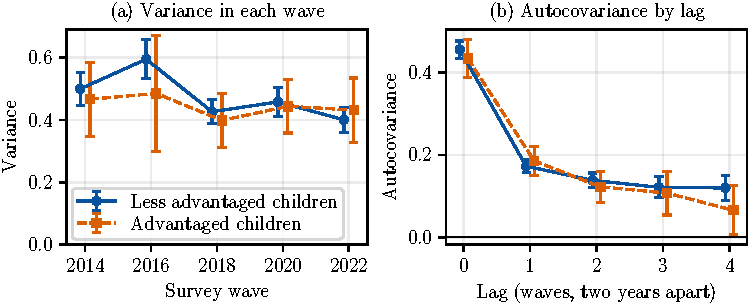
\includegraphics[width=0.78\textwidth]{figures/fig_autocov}
\caption{The second moments of residual log earnings by family background. Variance in each wave (panel a) and autocovariance by lag, averaged over waves (panel b), for advantaged and less advantaged children, with 95 percent bootstrap intervals (200 replications, clustered on person). The 2,523 children with at least three waves; residuals are demeaned within group and
year (wave sizes 1,319, 1,049, 2,197, 2,083, and 2,001). Averages over waves weight each wave pair by the inverse of its
bootstrap variance. Intervals overlap at every lag; the longest lags decide the permanent--transitory split of Table~\ref{tab:md}.}
\label{fig:autocov}
\end{figure}

\subsection{Persistence by dynamic panel GMM}
\label{sec:abgmm}

A dynamic panel regression gives a second estimate of transitory
persistence. Both estimators target the persistence of the transitory component, not that of observed residual earnings: the minimum-distance fit attributes part of the autocovariance to a permanent effect before fitting the decay, and the dynamic panel regression differences the permanent component away. Because both target the same parameter, a disagreement between them would signal misspecification of the process rather than a difference in what is estimated. Residual earnings follow the autoregression
\begin{equation}
\tilde y_{it} = \rho_0\, \tilde y_{i,t-1}
 + \rho_1\, (\tilde y_{i,t-1} \times H_i) + \alpha_i + u_{it},
\label{eq:ab}
\end{equation}
in which the individual effect $\alpha_i$ absorbs the permanent
component; I use the first-differenced estimator of
\citet{ArellanoBond1991}, with lagged levels as instruments. Estimation is two-step GMM with cluster-robust two-step sandwich standard errors; the instruments are lags two and three, collapsed \citep{Roodman2009}. On the 2014--2022 panel the estimate for less advantaged children is
$\hat\rho_0 = 0.058$ (SE 0.036). The moment set passes the Hansen test and the test for second-order serial correlation; the diagnostics, and a system GMM estimate in the manner of \citet{BlundellBond1998} whose level moments the Hansen test rejects, are in the Online Appendix.
The two estimators agree: the minimum-distance estimate for less advantaged children, 0.12, lies inside the 95 percent interval of the Arellano--Bond estimate, $[-0.01, 0.13]$. The autocorrelation of observed residual earnings, which adds to this transitory persistence the permanent share of the remaining variance, is near 0.4 at the pooled estimates, more than twice the transitory parameter (Section H.7 of the Online Appendix).

The interaction of lagged earnings with family background is 0.009 (SE 0.094), with a Wald interval of $[-0.17, 0.19]$: persistence does not differ by family background. The interval excludes large group differences but not moderate ones (the smallest interaction the design detects with 80 percent power is 0.26).

\subsection{Nonlinear persistence, growth, and the group comparison}
\label{sec:abb}

Linear autoregressions average over a feature that
\citet{ArellanoBlundellBonhomme2017} document in American data: the
persistence of the earnings state depends on the worker's position in
the distribution and on the size of the shock. Their nonlinear state equation, fitted here by stochastic EM (Online Appendix), reproduces the pattern found in American data, and persistence averaged over a lattice of state and shock-rank quantiles is 0.46 in the pooled sample, 0.54 for advantaged children, and 0.44 for less advantaged children. The higher figure for advantaged children holds in each of ten runs of the estimator and has the same sign as the difference between the separate minimum-distance fits of Table~\ref{tab:md}; it too would be the opposite of protection. The state absorbs the permanent component, so these figures compare with the autocorrelation of observed residual earnings (Section~\ref{sec:abgmm}), not with the transitory parameter.

Advantaged children might instead have steeper earnings paths. A fixed-effects regression of residual earnings on the interaction of the group indicator with a linear trend,
\begin{equation}
\tilde y_{it} = \alpha_i + \gamma\,(H_i \times t) + \delta' z_{it} + e_{it},
\label{eq:fe}
\end{equation}
where $z_{it}$ collects the time-varying covariates, gives $\hat\gamma = 0.018$ per wave (cluster SE 0.014) on the five-wave panel and 0.015 (SE 0.008) on the reconstructed panel without the covariates. The point estimates imply a divergence of 0.09 and 0.08 log points over a decade, and neither differs from zero at the 5 percent level; on the five-wave panel the 95 percent interval runs from about $-0.05$ to 0.23 log points over a decade. The strict-exogeneity restriction behind the fixed-effects estimate passes the lead test of \citet[Section~10.7.1]{Wooldridge2010}, reported in the Online Appendix.

The absence of a growth gap fits the timing of the return to college: children are 31 on average in the first wave in which they are observed, and by then most of the return to college is already in the level of earnings (Section~\ref{sec:sample}), so it adds little to measured growth.

\begin{table}[t]
\centering
\small
\caption{Group comparison across process moments.}
\label{tab:summary}
\begin{tabular}{@{}lccc@{}}
\toprule
Moment & Advantaged & Less advantaged & Gap or test \\
\midrule
Fifteen variances and autocovariances, joint test of equality & \multicolumn{2}{c}{---} & $p = 0.32$ \\
Fitted total variance (minimum distance) & 0.438 & 0.460 & $-0.022$ \\
Transitory persistence, Arellano--Bond & 0.066 & 0.058 & $+0.009$ \\
 &  &  & (0.094) \\
Nonlinear persistence, average over quantiles & 0.54 & 0.44 & $+0.11$ \\
Differential growth per wave, fixed effects & \multicolumn{2}{c}{---} & $+0.018$ \\
 &  &  & (0.014) \\
\addlinespace
\multicolumn{4}{@{}l}{\emph{One process for both groups?}} \\
Common parameters versus separate fits (distance test) & \multicolumn{2}{c}{---} & $p = 0.39$ \\
Three parameter gaps of the separate fits (Wald test) & \multicolumn{2}{c}{---} & $p = 0.09$ \\
Scale of advantaged autocovariances, $\kappa$ & 0.96 & 1 & $[0.85, 1.07]$ \\
 & (0.07) &  &  \\
Gap with one parameter free: permanent variance $\sigma^2_\eta$ & \multicolumn{2}{c}{---} & $-0.010$ \\
 &  &  & (0.022) \\
Gap with one parameter free: transitory persistence $\rho_v$ & \multicolumn{2}{c}{---} & $+0.03$ \\
 &  &  & (0.08) \\
Gap with one parameter free: shock variance $\sigma^2_\varepsilon$ & \multicolumn{2}{c}{---} & $-0.019$ \\
 &  &  & (0.031) \\
\bottomrule
\end{tabular}

\par\smallskip
\begin{minipage}{0.92\textwidth}
\footnotesize\emph{Notes:} Compiled from Table~\ref{tab:md} and Sections~\ref{sec:abgmm} and \ref{sec:abb}; the first row is the joint Wald test of Section~\ref{sec:md}, and the last panel the joint fits of the two groups described there (the distance test recenters bootstrap moments on the common fit; the scale model lets every autocovariance of advantaged children be $\kappa$ times that of less advantaged children). The bracket in the $\kappa$ row is a 90 percent bootstrap interval; the nonlinear persistence row carries no standard error. Standard errors in parentheses where available. Gaps, and the Arellano--Bond estimate for advantaged children, are computed from unrounded estimates.
\end{minipage}
\end{table}

Table~\ref{tab:summary} collects the group comparison. Total variance,
the autocovariances, the dynamic panel autoregression, and average growth agree across the two groups, and a single process fits both groups as well as separate processes do. Growth also bears on timing: a premium measured on the level of earnings might be a starting gap that later growth would widen or close. To the extent that earnings grow at the same rate in both groups after the ages at which the level is measured, the level measured there is also the long-run level. Family background is associated with the level of earnings, not with the variance of earnings around that level or with its growth, so whatever advantage these families confer must already be in the level that Section~\ref{sec:premium} measured.

\subsection{What the process implies for measurement}
\label{sec:measurement}

The estimated process also shows how much a regression on a few waves of parental income understates its coefficient, and how many waves undo most of the bias. Let $y^*_i$ denote the permanent log income of the parents of child $i$
and suppose the researcher
observes $y_{iT} = y^*_i + \bar v_{iT}$, the average of $T$ waves of
parental income, which contains transitory variation. In a regression of a child
outcome on $y_{iT}$, the probability limit of the coefficient is the
true coefficient scaled by
\begin{equation}
\lambda_T \;=\; \frac{\sigma^2_\eta}
{\sigma^2_\eta + \sigma^2_\varepsilon / \big(T\,(1-\rho_v^2)\big)},
\label{eq:eta}
\end{equation}
treating the transitory components of the $T$ observed waves as mutually uncorrelated.\footnote{With biennial persistence $\rho_v = 0.16$ the exact variance of the $T$-wave average carries cross terms. The exact calculation, derived in Part II of the Online Appendix, lowers $\lambda_5$ from 0.65 to 0.59 and pushes the two-thirds crossing from six waves to eight, so the figures in the text, which use the simple formula, understate the attenuation.} Evaluated at the pooled estimates (Table~\ref{tab:eta}), the reliability ratio $\lambda_T$ is 0.27 at $T = 1$: a single wave recovers about a quarter of the coefficient on permanent income. Averaging helps quickly at first and slowly later. Recovering two thirds of the coefficient, about the share that \citet{Mazumder2005} finds short averages recover in the United States, takes about six biennial waves (eight under the exact calculation), a decade or more of panel coverage. A separate life-cycle correction applies in addition when income is observed far from mid-career
\citep{HaiderSolon2006}; the schedule here concerns panel length, not
observation age. 

\begin{table}[t]
\centering
\small
\caption{The attenuation schedule at the estimated parameters.}
\label{tab:eta}
\setlength{\tabcolsep}{3pt}
\begin{tabular*}{0.98\textwidth}{@{\extracolsep{\fill}}lccccccc@{}}
\toprule
\multicolumn{8}{@{}l}{\emph{Share of the coefficient on permanent income recovered by an average of $T$ waves}} \\
Waves averaged $T$ & 1 & 2 & 3 & 4 & 5 & 6 & 7 \\
\midrule
Reliability ratio $\lambda_T$, independence approximation & 0.27 & 0.43 & 0.53 & 0.60 & 0.65 & 0.69 & 0.72 \\
Reliability ratio $\lambda_T$, exact & 0.27 & 0.39 & 0.48 & 0.54 & 0.59 & 0.63 & 0.66 \\

\bottomrule
\end{tabular*}
\par\smallskip
\begin{minipage}{0.98\textwidth}
\footnotesize\emph{Notes:} Equation~\eqref{eq:eta} at the pooled
estimates $\sigma^2_\eta = 0.125$, $\sigma^2_\varepsilon = 0.326$, $\rho_v = 0.16$. The exact row replaces the independence approximation
with the full variance of a $T$-wave average of serially correlated
transitory components. 
\end{minipage}
\end{table}

Applied to a published study that uses the same survey, the schedule closes part of the gap between its raw and its preferred estimates: under the parents' process, between a quarter and just under one half. \citet{FanYiZhang2021} use its 2010 to 2016 waves, with income averaged over two to four biennial waves; divided by the shares that such averages recover, their raw least squares estimates of the intergenerational income elasticity imply a true coefficient between 0.31 and 0.45 under the children's process, an interval that contains their preferred estimates. The parents' own process matters here: the linked parents have a permanent share of 0.43 against 0.27 for the children, so a single wave of their income recovers a little over two fifths of the coefficient and the implied coefficient is $[0.22, 0.30]$. The Online Appendix gives the calculation, the raw and preferred estimates, and the attenuation of rank-based measures.

\section{The college channel: the 1999 expansion}
\label{sec:expansion}

Section~\ref{sec:premium} measured a premium in the level of earnings with parental income held fixed, and Section~\ref{sec:process} found no sign of it in the earnings process. This section asks how much of it runs through college, in the two steps of identity~\eqref{eq:hp-intro}: Section~\ref{sec:firststage} estimates, by family background, which children entered college because of the seats added in the 1999 expansion, and Section~\ref{sec:earnings} estimates what a degree did to the earnings of those children. The instrument, the design, and the threats to it come first (Section~\ref{sec:design}).

\subsection{Design and threats}
\label{sec:design}

Following \citet{Duflo2001}, the design instruments college completion $M_i$ (sixteen or more years
of schooling) with provincial intensity multiplied by cohort exposure,
$Z_i = \mathrm{Intensity}_{p(i)} \times \mathrm{Exposure}_{c(i)}$. The outcome is the level of earnings (Section~\ref{sec:sample}). The conventional regression has one observation for each of the 2,774 children who have a level of earnings, $\bar y_{io}$ (the subscript $o$ marks earnings at ages 30 and over):
\begin{equation}
\begin{aligned}
\bar y_{io} &= \beta_o M_i + \theta_1 H_i + \delta' X_i + \mu_{p(i)} + \mu_{c(i)} + e_{i}, \\
M_i &= \pi_o Z_i + \psi_1 H_i + \gamma' X_i + \mu_{p(i)} + \mu_{c(i)} + u_i,
\end{aligned}
\label{eq:oldonly}
\end{equation}
where $X_i$ contains $\pinc_i$, gender, and urban residence, $\mu_{p(i)}$ are province
effects, and $\mu_{c(i)}$ is one effect per birth year. The coefficient $\beta_o$ is the return to college in the level of earnings, and $\pi_o$ is its first-stage coefficient.

The main specification adds a second row to this regression. Equation~\eqref{eq:oldonly} leaves out the 1,762 children who are not yet 30 or have fewer than two waves at 30 and over, although they belong to the same provinces and birth cohorts and carry information on the province effects, the birth-year effects, and the coefficients on the controls. The gain from using them is largest for the estimates by family background, whose birth-year effects are specific to each group and rest on few advantaged children. I therefore give each child up to two rows. The row at 30 and over holds $\bar y_{io}$, a mean over at least two waves because transitory variance is three quarters of the variance of earnings in a single wave (Section~\ref{sec:measurement}). The row below 30 holds $\bar y_{ib}$, the same mean over the child's waves at ages 22 to 29, when the child has at least one such wave (2,774 and 2,343 rows). Let $r \in \{o, b\}$ index the rows of child $i$ and let $O_r$
equal one for the row at 30 and over. The two-row specification is
\begin{align}
\bar y_{ir} &= \beta_o\, M_i O_r + \beta_b\, M_i (1 - O_r) + \theta_1 H_i
+ \theta_2 H_i O_r + \theta_3 O_r + \delta' X_i + \mu_{p(i)} + \mu_{c(i)} +
e_{ir}, \label{eq:twoband} \\
M_i O_r &= \pi_o\, Z_i O_r + \pi_{b}\, Z_i (1 - O_r) + \psi_1 H_i
+ \psi_2 H_i O_r + \psi_3 O_r + \gamma' X_i + \mu_{p(i)} + \mu_{c(i)} +
u_{ir}. \label{eq:fso}
\end{align}
College completion enters equation~\eqref{eq:twoband} separately for the two rows, and each of the two terms has its own instrument: $M_i O_r$ is instrumented by $Z_i O_r$ and $M_i (1 - O_r)$ by $Z_i (1 - O_r)$. Equation~\eqref{eq:fso} is the first stage for $M_i O_r$; the one for $M_i (1 - O_r)$ has the same form. The coefficient $\theta_3$ lets mean earnings differ between the rows, and $\theta_2$ lets the premium differ between them; the province effects, the birth-year effects, and the coefficients on $X_i$ are common to the two rows.

Three coefficients carry the results: the return $\beta_o$, its first-stage coefficient $\pi_o$, and its reduced form, the coefficient on $Z_i O_r$ in the regression of $\bar y_{ir}$ on the two instruments and the controls. As in equation~\eqref{eq:oldonly}, $\beta_o$ is the return to college in the level of earnings, and the conventional regression gives nearly the same value (0.70 against 0.68, Section~\ref{sec:earnings}). I do not report or interpret $\beta_b$: every child observed below 30 between 2014 and 2022 was born in
1985 or later and reached college age well after the expansion had begun, so the reform does not identify it.

Two variants show what the second row and the equal weighting of rows contribute: the conventional regression of equation~\eqref{eq:oldonly}, and a regression that keeps both rows and weights them by precision. The rows are means of different numbers of waves, and under equation~\eqref{eq:feAR}, with a child's transitory components treated as uncorrelated as in equation~\eqref{eq:eta}, the mean of $n_{ir}$ waves has variance $\sigma^2_\eta + \sigma^2_v / n_{ir}$, the denominator of equation~\eqref{eq:eta} with $n_{ir}$ in place of $T$; the weight of a row is its inverse,
\begin{equation}
w_{ir} \;=\; \left( \hat\sigma^2_\eta +
\frac{\hat\sigma^2_\varepsilon}{(1 - \hat\rho_v^2)\, n_{ir}}
\right)^{-1},
\label{eq:weights}
\end{equation}
evaluated at the pooled estimates of Table~\ref{tab:md} ($\hat\sigma^2_\eta = 0.125$, $\hat\sigma^2_\varepsilon = 0.326$, $\hat\rho_v = 0.16$). The same three parameters do two jobs: in Section~\ref{sec:measurement} they say how much a noisy regressor attenuates a coefficient, and here they say how precisely an average of earnings measures an outcome. I keep the unweighted regression as the main specification because it does not depend on the fitted process, and Section~\ref{sec:earnings} reports the
weighted one beside it.

Each child is assigned the province of residence in the first wave observed at ages 22 to 55, and the birth year that wave implies, as a proxy for the province of examination registration, which CFPS does not record. A child who moved before that wave is assigned the wrong intensity, which attenuates provincial contrasts. Such moves are uncommon and no more common in one group than in the other: of the 2,578 children for whom the 2010 wave records the province of residence at age twelve, 8 percent of advantaged children and 7 percent of less advantaged children are assigned a different province. Section~\ref{sec:earnings} reports the estimates with the instrument assigned by the province at age twelve.

The model is exactly identified, with one excluded instrument
for each endogenous regressor, and
two-stage least squares and LIML coincide. Intensity varies at
the province level, so inference rests on 29 clusters. I
report wild cluster bootstrap $p$-values \citep[Rademacher weights by
province, null imposed, 9,999 replications;][]{CameronGelbachMiller2008} and wild cluster
Anderson--Rubin sets for the instrumented returns to college. These procedures do not need many clusters: the bootstrap imposes the null, the Anderson--Rubin sets stay valid under a weak first stage, and the randomization test below needs no asymptotic approximation at all; all three agree. Randomization inference, which reassigns the 29 provincial values of intensity at random among the provinces, gives $p < 0.001$ for the earnings reduced form and for the first stage, whether intensity is reassigned among all provinces or only within regions (Online Appendix). The
two rows of a child lie in the same province, so clustering on province
allows for their correlation.

I measure first-stage strength by the cluster-robust $F$ on $Z_i O_r$ in equation~\eqref{eq:fso}, the one instrument that is not zero on the rows at 30 and over (in the conventional regression it is the effective $F$ of \citet{OleaPflueger2013}). Birth-year effects absorb the national path of admissions; the estimates rest on the remaining 14 percent of the instrument's variance net of province effects, the interaction of provincial intensity with cohort exposure.

Identification is that of an exposure design, the exogenous-shares case of
\citet{GoldsmithPinkham2020} with provincial intensity as the single share and cohort exposure as the shift: provincial intensity must be unrelated to
province-by-cohort shocks to the outcomes, conditional on province and
cohort means. Province fixed effects absorb any time-invariant relation
between intensity and outcome levels (high-intensity provinces are
richer on average), so the remaining threats are trending confounders.
Provinces with rapid pre-reform growth in examination demand might be on differential trends more generally. The placebo instrument built from pre-reform growth in examination registrations has no first stage (Table~\ref{tab:threats}). Registrations are upstream of admissions, so the placebo picks up any provincial trend in the demand for college but not the reform; a placebo with no first stage means that the instrument follows the seats that were added rather than a trend.

Exclusion requires that the instrument move the outcomes only through
college, conditional on the controls; the main
competing shock of the period is WTO accession, whose provincial
geography could correlate with provincial intensity. The expansion also enlarged the supply of graduates, which lowered the relative wages of graduates in the cohorts entering the labor market \citep{KnightDengLi2017}; to the extent that graduates work where they studied, their lower relative wages push the earnings reduced form toward zero, so the return estimated here is, if anything, understated. Table~\ref{tab:threats} lists each assumption with its main threat, the checks I run, and their results (Section~\ref{sec:earnings}).

\begin{table}[t]
\centering
\footnotesize
\caption{Identifying assumptions, threats, and diagnostics.}
\label{tab:threats}
\begin{tabular}{@{}L{2.8cm}L{3.9cm}L{8.0cm}@{}}
\toprule
Assumption & Principal threat & Diagnostic and result \\
\midrule
Instrument relevance & Weak first stage in a group or under another intensity measure
& First-stage $F$ of 18.0 for all children, 16.9 and 12.3 by family background, and 13.3 to 39.8 under the three other measures (Table~\ref{tab:groups} and the Online Appendix) \\
\addlinespace
Exclusion: the instrument reaches earnings only through college & A shock of the reform years, such as trade after WTO accession, that is correlated with intensity and reaches earnings outside college &
Trade-exposure controls: reduced form 0.127 to 0.140, against 0.128. Children with nine or fewer years of schooling: occupation 0.017 (SE 0.019). Reduced form of the child's adult urban residence: 0.006 (SE 0.022) \\
\addlinespace
Parallel trends: provincial intensity unrelated to province-by-cohort shocks & Provinces that added more seats were already on different trends &
Placebo from pre-reform registration growth: first-stage $F$ of 0.5. Predetermined census measure: return 0.67. Cohorts born in 1980 or earlier: no trend in earnings or completion ($p = 0.56$ and $0.75$). Linear cohort trends by region: return 0.72. Census cohorts before the reform: under one percentage point of divergence over 20 cohorts \\
\bottomrule
\end{tabular}
\par\smallskip
\begin{minipage}{0.95\textwidth}
\footnotesize\emph{Notes:} Estimates for the row at 30 and over of equation~\eqref{eq:twoband} under the main measure of intensity unless the entry names another measure; standard errors clustered on province; $p$-values are wild cluster bootstrap $p$-values; reduced forms are coefficients on the instrument in regressions of the named outcome on the instrument and the controls.
\end{minipage}
\end{table}

\subsection{First stages and whom the reform moved}
\label{sec:firststage}

The gap in college completion between the two groups can be read in two ways, as the introduction set out: the examination score that rationed seats may have ranked ability alone or preparation under unequal conditions. Both readings imply that added seats admitted children from below the old cutoff; they differ in what college added to those children's earnings. Panel (a) of Figure~\ref{fig:fs} plots the college completion rate by family background in five groups of birth cohorts: completion rose across the reform from 17.3 to 50.5 percent among advantaged children and from 4.6 to 24.2 percent among less advantaged children, and the ratio of the two rates, printed under each group of cohorts, falls across the five groups. These are changes across cohorts with the national expansion included; what the added seats did is the question for the first stage, which panel (b) shows as a binned scatter for each group.

\begin{figure}[t]
\centering
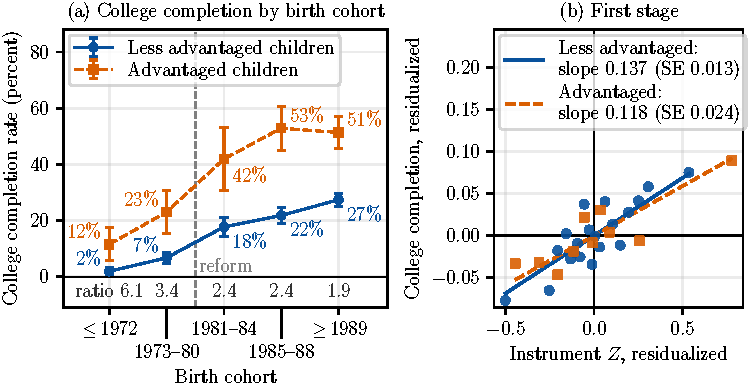
\includegraphics[width=0.84\textwidth]{figures/fig_first_stage}
\caption{College completion by family background and the first stage. Panel (a): college completion rate by family background in five groups of birth cohorts, with 95 percent intervals from the binomial standard error; the number under each group is
the ratio of the rate of advantaged children to the rate of less
advantaged children. Panel (b): binned scatter (20 bins of less advantaged and 10 bins of advantaged children) of college completion on the instrument by family background, in the
regression with province effects common to the two groups and
birth-year effects specific to each; both variables are residualized on
the other group's instrument and the controls, and the lines have the group first-stage slopes with province-clustered standard errors. All 4,536 children in the sample, one observation per child.}
\label{fig:fs}
\end{figure}

On all 4,536 children, one observation per child, the main intensity measure gives a first-stage coefficient of 0.136 ($F = 102.9$): relative to the cohorts born before 1981, moving from a province at the 10th percentile of intensity to one at the 90th raises the college completion of a cohort born in 1989 or later by 18 percentage points. The first stage behind the returns of Section~\ref{sec:earnings}, on the rows at 30 and over, is 0.186 (SE 0.044) with $F = 18.0$; it is weaker because it rests on the 2,774 children already observed at those ages. The three other measures of intensity also have strong first stages (Online Appendix).

To estimate the first stage by family background I let the instrument enter separately for the two groups in one regression, with birth-year effects specific to each group, so that each group's national rise in completion is removed separately, and province effects common to the groups, because the advantaged children, 755 in all and 453 with a level of earnings, are too few for a separate set (Online Appendix). On all children the first-stage coefficient is 0.137 for less advantaged children and 0.118 for advantaged children (Figure~\ref{fig:fs}), and the difference between them, $-0.019$ (SE 0.019), is not distinguishable from zero. These coefficients are responses to provincial seat growth net of the national trend: the added seats gave children in both groups a similar chance of entering college (18 and 15 percentage points for the same difference in intensity). Given a pre-reform ratio of completion rates of 3.7 to one in favor of advantaged children, the added seats were a step toward equal access: relative to the groups' pre-reform rates, an addition of similar size is a far larger proportional change for less advantaged children, so it narrowed the gap as a ratio while leaving it roughly unchanged in percentage points. The first stages on the rows at 30 and over are again not distinguishable between the groups (Online Appendix).

The first stage identifies the allocation of the seats that provinces added beyond the national path, not that of the national expansion itself. The similar first stages imply that, across provinces, the gap in percentage points widened by about as much where few seats were added as where many were. Across cohorts, with the national expansion included, the ratio fell from 3.7 to 2.1 and the gap in percentage points widened from 13 to 26. Both changes lie in the national rise of admissions, which the birth-year effects absorb (the Online Appendix sets out the arithmetic). The first stage says which children the added seats admitted; what college returned to them, on which the two readings differ, is the question of Section~\ref{sec:earnings}.

\subsection{What college returned: earnings and occupation}
\label{sec:earnings}

This subsection estimates what a four-year degree did for the children the added seats admitted: first for their level of earnings, which is the return to college that identity~\eqref{eq:hp-intro} needs, since the premium is a gap in that level, and then for their occupation. The specification is the two-row regression of
equation~\eqref{eq:twoband}, and, unless noted, every estimate below is the one for the row at 30 and over; the cohorts born before 1981 supply the earnings
gradient on provincial intensity in the absence of the reform.

Under the main measure of intensity (Table~\ref{tab:groups}), on the rows at 30 and over, moving from the 10th to the 90th percentile of intensity raises the completion of the most exposed cohorts by 24 percentage points and their level of earnings by about 18 percent. The instrumented return to college is 0.68 log points, against a least squares return of 0.45, and the 95 percent wild cluster Anderson--Rubin set, $[0.50, 4.20]$, excludes zero and the least squares return. Inverting the randomization test under a common return, with reassignment within regions, gives a narrower 95 percent set, $[0.45, 1.30]$; the set is narrower because it imposes a common return and treats intensity as exchangeable across provinces, not because it is more reliable.

The three other intensity measures give returns of 0.63 to 0.72 (Online Appendix). The census measure is fixed in every component before the reform, so its agreement with the main measure, whose denominators date from after it, addresses the concern that the expansion itself shaped the intensity it is instrumented with. Table~\ref{tab:threats} collects the checks on exclusion and parallel trends. Children with nine or fewer years of schooling, who were never candidates for college, did not move into official, managerial, or professional occupations where seats grew faster. The trade-exposure controls, cohort exposure interacted with a coastal indicator and with the province's export share, leave the reduced form in place. The child's urban residence in adulthood, a route to higher earnings outside college, does not move with the instrument. Dropping one province at a time gives returns between 0.65 and 0.73, except for Shanghai, the province with the highest intensity: without it the reduced form stays at 0.125, the first stage falls to 0.112, and the return is 1.11, with an Anderson--Rubin set that starts at 0.55. Figure~\ref{fig:mature} reports the event study: the earnings gradient on provincial intensity is flat across the pre-reform cohort bins, the completion gradient is not distinguishable from zero at the 5 percent level in either bin, and both rise across the three post-reform bins with the exposure of the cohort.

\begin{figure}[t]
\centering
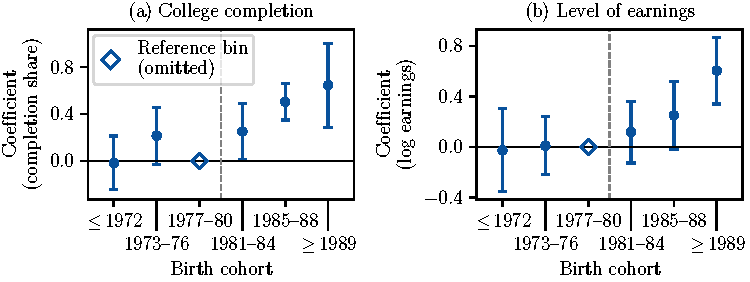
\includegraphics[width=0.84\textwidth]{figures/fig_mature_age}
\caption{Event study: completion and earnings gradients on provincial intensity by birth cohort. College completion (panel a) and the level of earnings (panel b) by cohort bin: coefficients on
interactions of provincial intensity with the birth-cohort bins
1972 or earlier, 1973--1976, 1981--1984, 1985--1988, and 1989 or later, with the reference bin 1977--1980 plotted at zero. Main intensity measure; the 2,774 children with a level of earnings, one observation per child on the rows at 30 and over, unweighted; demographic controls, birth-year effects, and province effects included; 95 percent intervals clustered on province. Coefficients are per unit
of provincial intensity and are not comparable with the first-stage
coefficient on $Z$. The dashed line marks the reform.}
\label{fig:mature}
\end{figure}

The return changes little with regional cohort trends, with the instrument assigned by the province at age twelve, and with cohort exposure taken at age seventeen or nineteen instead of eighteen (0.64 to 0.74). A linear cohort trend for each province gives 0.77, with a reduced form of 0.100 (SE 0.065), and leaving out the cohorts born 1973 to 1976 gives 0.60. Among the cohorts born in 1980 or earlier, neither earnings nor completion trends with provincial intensity, and in the 1990 and 2000 census microdata \citep{IPUMSInternational}, which cover cohorts past college age before the reform, the cohort slope of university completion differs between provinces in the top and bottom terciles of intensity by under one percentage point over 20 cohorts. Dropping the second row (equation~\eqref{eq:oldonly}) gives a return of 0.70, and weighting the rows by the precision of equation~\eqref{eq:weights} gives 0.63. The Online Appendix reports these and further checks.

\begin{table}[t]
\centering
\small
\caption{First stages, earnings reduced forms, and returns to college, for all children and
by family background.}
\label{tab:groups}
\setlength{\tabcolsep}{4pt}
\begin{tabular}{@{}lccccccc@{}}
\toprule
& & First & Earnings & Instrumented & \multicolumn{2}{c}{Anderson--Rubin set} & Least \\
\cmidrule(lr){6-7}
& Children & stage & reduced form & return & 95 percent & 90 percent & squares \\
\midrule
All children & 2,774 & 0.186\rlap{**} & 0.128\rlap{***} & 0.68 & $[0.50, 4.20]$ & $[0.55, 2.30]$ & 0.45 \\
 &  & (0.044) & (0.018) &  &  &  & (0.038) \\
 &  & $F$ = 18.0 & [0.002] &  &  &  &  \\
\addlinespace
Less advantaged & 2,321 & 0.182\rlap{**} & 0.115\rlap{***} & 0.62 & $[0.45, 4.45]$ & $[0.45, 2.30]$ & 0.44 \\
 &  & (0.044) & (0.018) &  &  &  & (0.039) \\
 &  & $F$ = 16.9 & [0.004] &  &  &  &  \\
\addlinespace
Advantaged & 453 & 0.189\rlap{*} & 0.191\rlap{**} & 1.14 & $(-\infty, -0.50]$ & $(-\infty, -3.20]$ & 0.51 \\
 &  & (0.054) & (0.058) &  & $\cup\ [0.25, \infty)$ & $\cup\ [0.60, \infty)$ & (0.059) \\
 &  & $F$ = 12.3 & [0.042] &  &  &  &  \\
\bottomrule
\end{tabular}

\par\smallskip
\begin{minipage}{0.92\textwidth}
\footnotesize\emph{Notes:} Two-row specification of equation~\eqref{eq:twoband} on all 4,536 children in the sample; every entry is the estimate for the row at 30 and over, and Children is the number of such rows, one per child with a level of earnings.  Second and third rows: one regression for each column of estimates, with the instrument entering separately for each group and row, province effects common to the groups, birth-year effects specific to each group, and the controls of equation~\eqref{eq:twoband}. Province-clustered standard errors in parentheses. Below each first-stage standard error is its cluster-robust $F$ statistic; below each reduced-form standard error, in brackets, is its wild cluster bootstrap $p$-value. The Anderson--Rubin sets invert the wild cluster bootstrap test over returns from $-6$ to 6 in steps of 0.05, and a set is reported as unbounded when the test does not reject at the end of the grid, which happens when it does not reject a zero first stage for the group's own college completion at that level. Because province effects are common to the groups, the two returns by family background are estimated jointly, and neither equals the ratio of the group's reduced form to its first stage. Least squares: the coefficient on college completion in the same rows. *, **, and *** denote significance at the 10, 5, and 1 percent levels by the wild cluster bootstrap $p$-value (not printed for the first stage).
\end{minipage}
\end{table}

Counted over the four years of a degree, the instrumented return of 0.68 is about 0.17 log points (19 percent) per year of college. This is close to what other designs find for China: near 10 percent per year of schooling in urban China around 2000 \citep{ZhangZhaoParkSong2005, HeckmanLi2004}, 12 to 17 percent per year with an instrument that combines the expansion with childhood household registration \citep{HuangTaniWeiZhu2022}, and about 20 percent per year with the 1986 compulsory schooling law \citep{FangEtAl2012}.

Table~\ref{tab:groups} sets the return for all children beside the returns by family background, each with its Anderson--Rubin sets and its least squares benchmark. Both groups have a first stage, and both earnings reduced forms are positive and significant at the 5 percent level by the wild cluster bootstrap. The instrumented return is 0.62
for less advantaged children and 1.14 for advantaged children; the least squares returns are 0.44 and 0.51. For less advantaged children the 95 percent Anderson--Rubin set is $[0.45, 4.45]$; the set for advantaged children is unbounded on both sides. The estimates point to a higher earnings return to college for advantaged children, though the difference is within sampling error ($z = 1.41$, which accounts for the covariance of the two estimates); neither point estimate is below the least squares return. A difference in these returns, were it established, would be a difference in the level of earnings that a degree delivers, not in the earnings process of Section~\ref{sec:process}; Section~\ref{sec:mediation} counts it in the direct effect, as the extra value of a degree to an advantaged child.

\label{sec:occupation}
The earnings gain has an occupational counterpart. The premium is
defined by parental occupation, so I ask whether the expansion moved
children into official, managerial, or professional occupations of
their own, which I call advantaged occupations for short. The outcome
is the share of the child's waves at ages 30 and over in which the
reported occupation belongs to CSCO major groups 1 or 2, in the two-row regression of equation~\eqref{eq:twoband} with the share below 30 as the second row; it is the chance of holding such an occupation at a given wave. Its reduced form on the instrument is 0.092 (wild cluster $p = 0.016$), which implies that college raises the share of those waves spent in an advantaged occupation by 0.50, or 50 percentage points; the three other intensity measures give reduced forms of the same sign (Online Appendix).

A degree also closes the occupational gap between the groups. Among the 2,762 children with at least two waves at ages 30 and over that report an occupation, advantaged children spend twice the share of those waves in an advantaged occupation (0.33 against 0.17), and about twice the share among children without a degree (0.19 against 0.10); among graduates, the two groups spend the same share (0.60 each). With parental income and demographics held fixed by entropy balancing, the shares are 0.60 against 0.59 among graduates (95 percent bootstrap interval of the gap $[-0.08, 0.11]$) and 0.19 against 0.14 among children without a degree ($[0.01, 0.10]$).

By family background, in the regression of Table~\ref{tab:groups}, the point estimates place the larger occupational gain with less advantaged children: college raises their share of waves in an advantaged occupation by 0.55 (SE 0.24), against 0.13 (SE 0.31) for advantaged children, whose reduced form is not distinguishable from zero. The difference is within sampling error ($z = 1.25$) and runs opposite to the difference in earnings returns. The estimates by family background are therefore suggestive rather than settled. The sample establishes the return for all children; whether a degree returns more to an advantaged child, the interaction of family background with college completion, it can neither confirm nor rule out, so Section~\ref{sec:mediation} evaluates the identity at the return for all children as well as at the return for advantaged children.

The completion indicator counts four-year degrees only. Completion of a three-year degree does not rise with the instrument (coefficient $-0.06$, SE 0.03, wild cluster $p = 0.29$), so the reduced form carries no earnings effect of added three-year degrees. If some of the children who completed a four-year degree because of the added seats would otherwise have held a three-year one, 0.68 compares a four-year degree with a mix of no college and a three-year degree.

Under monotonicity (more seats in the province make no child less likely to complete college), the instrument recovers a local average treatment effect in the sense of \citet{ImbensAngrist1994}: a weighted average of the returns to college for compliers, the children whom added seats moved into a four-year degree, drawn from the two groups roughly in proportion to their numbers in the sample, since a similar share of each group complied (Section~\ref{sec:firststage}). For all children, the point estimate (0.68) and the lower end of the 95 percent Anderson--Rubin set (0.50) lie above the least squares return (0.45, SE 0.04): the children whom the seat constraint had kept out earned at least as much from college as the earnings difference between graduates and other children would suggest. If the least squares return carries positive selection among the earlier graduates, as the first reading itself asserts, a return no lower than it is also no lower than what college returned to them. An instrumented return above the least squares return is the usual finding when an instrument relaxes a constraint on schooling \citep{Card2001}, and the usual explanation, a higher return for the children whom the constraint had kept out, is the second reading of Section~\ref{sec:firststage} rather than an alternative to it. If the examination had ranked preparation rather than ability, the children admitted under a lower cutoff could earn as much from the same college education as those admitted before them, or more.

\section{Decomposing the premium}
\label{sec:mediation}

The paper has measured three things on the level of earnings of the same 2,774 children: the premium, the gap in college completion, and the return to college. Identity~\eqref{eq:hp-intro} puts them together: the premium ($\tau$) equals the gap in college completion between the two groups ($\Delta M$), measured in the same comparison, valued at what a degree is worth to an advantaged child ($\beta^{H}$), plus a direct effect (Direct); the completion gap valued at that return is the college channel. With $\beta^{H}$ measured as the earnings difference between advantaged graduates and advantaged children without a degree, the equation holds exactly. Evaluated at a return estimated elsewhere, by regression or by the instrument, the identity values the completion gap and leaves a remainder, which Table~\ref{tab:bounds} reports as the direct effect; it equals Direct when that return equals $\beta^{H}$ and otherwise also contains the difference between the two returns times $\Delta M$ (Section I of the Online Appendix). Direct itself is the premium that would remain if the completion rate of advantaged children were lowered to that of less advantaged children. It collects the earnings gap between the two
groups among children without a degree and any difference between the
groups in the return to a degree, weighted by the completion rate of
less advantaged children \citep{HeckmanPinto2015}. 

Section~\ref{sec:premium} supplies the left side and the completion gap. Of the 0.195 log points (22 percent) by which advantaged children out-earn less advantaged children, 0.123 reflects parental income together with the demographic and provincial controls, and the remaining 0.072 (7 percent) is the premium $\tau$ with parental income held fixed. The completion gap is $\Delta M = 0.122$. Both come from the entropy-balanced
comparison of Section~\ref{sec:ebal} and not from the regressions,
because the identity is an equality between the means of two groups and
holds only if both sides are measured on the same two groups. Balancing
gives one comparison group, the less advantaged children reweighted to match the parental income and demographics of advantaged children, and the earnings gap and the completion gap are both taken against it. $\Delta M$ is the gap among all 2,774
children with a level of earnings, the cohorts before and after the reform together, because the
premium it has to account for is the earnings gap among all of them.
The expansion enters the identity in one place only, as the source of
the return. The Online Appendix gives the college share at the two regression estimates of the premium.

The least squares return compares graduates with children without a degree; the difference between the groups is not distinguishable from zero (Table~\ref{tab:groups}). Evaluated at a least squares return, the identity is an accounting exercise without a causal interpretation, and it reproduces a familiar regression: when the child's college completion is added to a least squares regression of the level of earnings on family background and the controls of equation~\eqref{eq:oldonly}, the coefficient on family background falls from 0.076 to 0.022, a drop of about the same share. The instrumented returns of
Section~\ref{sec:earnings} are returns for children who completed college because seats were added. All three point estimates, for all children and for each group, lie above the least squares returns, which I use as the other benchmark. The identity calls for the return for advantaged children: $\beta^{H}$ is the $\beta_o$ of Section~\ref{sec:design} estimated for them. Table~\ref{tab:bounds} evaluates the identity at their two returns and at the two returns for all children, which rest on six times as many children.

\begin{table}[t]
\centering
\small
\caption{The premium split into the college channel and the direct
effect, at alternative values of the return to college.}
\label{tab:bounds}
\setlength{\tabcolsep}{4pt}
\begin{tabular}{@{}lcccc@{}}
\toprule
& & College & Direct & College \\
Source of the return & Return to college & channel & effect & share \\
\midrule
Return at which college explains half of the premium & 0.294 & 0.036 & 0.036 & 0.50 \\
Least squares, all children & 0.449 & 0.055 & 0.017 & 0.76 \\
Least squares, advantaged children & 0.515 & 0.063 & 0.009 & 0.88 \\
Return at which college explains all of the premium & 0.588 & 0.072 & 0.000 & 1.00 \\
Instrumented, all children & 0.684 & 0.084 & $-0.012$ & 1.16 \\
Instrumented, advantaged children & 1.143 & 0.140 & $-0.068$ & 1.94 \\
\bottomrule
\end{tabular}
\par\smallskip
\begin{minipage}{0.9\textwidth}
\footnotesize\emph{Notes:} Level of earnings (2,774 children). The premium with parental income held fixed is 0.072 and the completion gap 0.122, both from entropy balancing
(Section~\ref{sec:ebal}). The college channel is the return times the completion gap, the direct effect is the premium minus the college channel, and the college share is the college channel divided
by the premium. A negative direct effect means that the completion gap valued at that return exceeds the premium: the return lies above 0.588, the return at which the direct effect is zero, and the Anderson--Rubin sets of both instrumented returns contain 0.588; the set for advantaged children is unbounded on both sides (Table~\ref{tab:groups}). All entries are computed from unrounded values. Instrumented and least squares returns from Table~\ref{tab:groups}, printed here to three decimals.
\end{minipage}
\end{table}

At the least squares returns the completion gap accounts for three quarters of the premium (the return for all children) and seven eighths (the return for advantaged children). College explains half of the premium at a return of 0.29 and all of it at 0.59 (Table~\ref{tab:bounds}). Both least squares returns lie between these two values, both instrumented returns lie above 0.59, and at 0.50, the lower end of the 95 percent Anderson--Rubin set for all children, the completion gap still accounts for 85 percent. Valued at what college returned to the children the expansion admitted, the completion gap accounts for all of the premium. This valuation treats the degrees that advantaged children hold in excess of less advantaged children as worth what a degree returned to the children the added seats admitted. Many of those degrees were completed before the reform; if their holders earned no more from college than the children admitted later, which is the second reading of Section~\ref{sec:firststage}, the instrumented return values the completion gap at or above its worth. Neither benchmark is the return to the extra degrees of advantaged children, and least squares is not a lower bound on it: with positive selection into college it overstates what a degree returned to its holders, and at lower returns the share falls below three quarters, to one half at 0.29.

With a separate return for each group, the identity is an Oaxaca--Blinder decomposition with college completion as the only covariate, evaluated at the coefficients of advantaged children \citep{Oaxaca1973, Blinder1973}. Inside the balanced comparison every term is a mean of the reweighted sample, so the three parts add up to the premium by construction; because the comparison group is reweighted rather than modeled, no regression and no residual enter the decomposition. Graduates out-earn children without a degree by 0.541 log points among advantaged children and by 0.517 among reweighted less advantaged children; these are raw differences inside the balanced comparison, whereas the least squares returns of Table~\ref{tab:bounds} add the controls of equation~\eqref{eq:oldonly}. The premium of 0.072 has three parts, each given here with a 95 percent bootstrap interval (1,000 replications that resample children within group and solve the weights again). The first, 0.066 ($[0.04, 0.09]$), comes from the degrees that advantaged children hold in excess
of less advantaged children, valued at the return for advantaged children;
it is the college channel, 92 percent of the premium. The second, 0.005 ($[-0.02, 0.04]$), comes from the degrees
that both groups hold (21 percent of each), which are worth slightly more to advantaged children. The third, 0.001 ($[-0.08, 0.07]$), is the gap between children of the two groups without a degree. The second and third parts are also where ability rewarded outside college would appear: if advantaged children were the more able at each level of schooling, they would out-earn less advantaged children with the same schooling. With parental income held fixed, they do not among children without a degree and barely do among graduates, where the gap is 0.024 log points ($[-0.09, 0.13]$) and the chance of holding an advantaged occupation is the same (Section~\ref{sec:earnings}). The second part is small, and whether a degree is worth more to an advantaged child is the question the returns by family background leave open (a difference within sampling error, Section~\ref{sec:earnings}). Only the first part depends on who completes college. The second and the third make up the direct effect.

College enters as a binary completion
indicator, so any advantage in college quality that is correlated with
family background is counted in the direct effect and not in the
college channel; if advantaged families, whose college completion was
already high, responded to the expansion by seeking better institutions \citep{LiuWan2019, LiuYueZhu2025},
the accounting understates the education system's role. The accounting measures how much of the premium is associated with completing college; whatever a degree carries with it, skills, credentials, connections, or access to urban labor markets, is counted with the degree.

The direct effect is also where an advantage built inside the labor market would have to appear, and Section~\ref{sec:process} found no sign of one in the earnings process. Taken together, the decomposition reduces what parental occupation passes on beyond income largely to one yes-or-no fact about a child, whether the child holds a four-year degree. That single fact accounts for between three quarters and all of the premium, a large share for so coarse a measure.

\section{Discussion and conclusion}
\label{sec:conclusion}

The earnings advantage of the children of officials, managers, and professionals is in place before they start work. I looked for its source in their earnings dynamics and found none. A single earnings process fits both groups as well as separate processes do: the variance of earnings, the persistence of shocks, and earnings growth do not differ between them. The same process also yields the attenuation factors that the literature on intergenerational persistence in China has lacked (Section~\ref{sec:measurement}).

With parental income held fixed, advantaged children earn 7 to 17 percent more, and the gap in college completion, valued at the return to college, accounts for between three quarters and all of this premium at its entropy-balanced value of 7 percent. The alternative reading, that officials, managers, and professionals have more able children, fails the tests of Sections~\ref{sec:earnings} and \ref{sec:mediation}. With parental income held fixed, children without a degree earn the same in the two groups; among graduates the earnings gap is small and the chance of holding an advantaged occupation is the same; and the children admitted only because seats were added earned no less from college than earlier graduates. Most of the advantage these families pass on beyond their income runs through access to college rather than through ability rewarded outside it.

Did the expansion pass inequality from one generation to the next, or open a door that family background had kept shut? The answer depends on the measure. In access, the door opened: completion among less advantaged children rose fivefold between the cohorts born in 1980 or earlier and those born later, the ratio of completion rates fell from 3.7 to 2.1, and the added seats gave children in both groups a similar chance of entering college. Those seats also reached children who could benefit from them: the instrumented return of less advantaged children, 0.62, is above their least squares return, 0.44, which suggests that unequal preparation rather than lesser ability had kept them below the cutoff. In the distance between the groups, inequality persisted: a similar addition to unequal starting points leaves the gap in percentage points roughly unchanged, and with the national rise in admissions that gap widened from 13 to 26 percentage points across cohorts, as earlier work on the expansion reports \citep{Yeung2013}.

The same two sides appear among those who came through the door. In occupation, it opened: advantaged children are twice as likely to hold advantaged occupations, overall and among children without a degree, but among graduates the two groups are equally likely to hold them, and for children who entered college because of the reform, the point estimates suggest a larger rise for less advantaged children. In earnings, some distance may remain: the same point estimates suggest a higher earnings return to college for advantaged children, and if that difference holds as more of the post-reform cohorts reach their thirties, part of the advantage of family background will have shifted from who completes college to what college returns. For the cohorts studied here, what parental occupation passes on beyond income is, for the most part, a single thing: a four-year degree. Family background shapes who holds one, and once children are at work, their earnings shocks and earnings growth no longer depend on it.

{\footnotesize
\setlength{\bibsep}{1pt}
\bibliography{refs}}

\end{document}
